\subsubsection{Desfibrilador}

A escolha do desfibrilador, para ser carregado no VANT foi realizada visto que:

\begin{citacao}
foi documentada uma taxa de 
sobrevivência entre vítimas de parada cardíaca com fibrilação ventricular confirmada acima de 90\% quando a desfibrilação é atingida
dentro do primeiro minuto de colapso. As taxas de sobrevivência declinam 7 a 10\% a cada minuto em que a desfibrilação
é atrasada, de modo que uma vítima de parada cardíaca sem desfibrilação por 12 minutos tem apenas 2 a 5\%
de chance de sobrevivência.\cite{1}
\end{citacao}

O objetivo em realizar a Reanimação Cárdio-Pulmonar (RCP) é prover oxigênio ao cérebro e coração até que
o tratamento adequado restaure os batimentos cardíacos normais, ou que permita o tempo necessário para a 
chegada de uma equipe de socorro de Suporte Avançado de Vida (SAV). Quando o início da RCP for retardado, 
a chance de sobrevida é prejudicada e o córtex cerebral (o tecido mais susceptível à lesão por baixa de 
oxigênio no sangue) sofre danos irreversíveis,resultando em morte ou seqüelas neurológica severa e permanente. \cite{2}

O desfibrilador externo automático (DEA) por ser portátil e automático, torna a possível utilização por 
pessoas sem formação médica, visto que ele possui um computador embutido que verifica o ritmo cardíaco da 
pessoa e calcula se a desfibrilação se faz necessária, mostrando um comando para a pessoa acionar o botão, de 
modo a liberar a carga no peito da vitima.\cite{3}. O diagrama de bloco mostrado na Figura \ref{fig:dea}, mostra todo o funcionamento do DEA.

\begin{figure}[h!]
	\centering
	  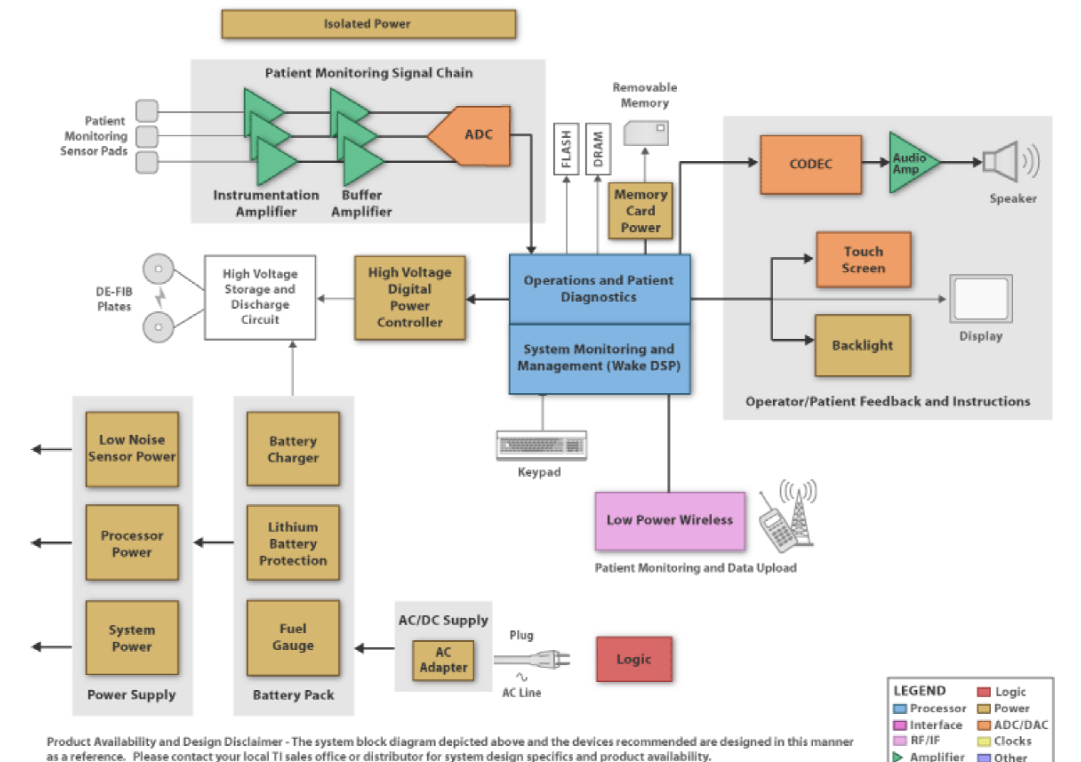
\includegraphics[keepaspectratio=true,scale=0.6]{figuras/dea.eps}
	\caption{Diagrama de Bloco. Fonte: \cite{bloco}}
	\label{fig:dea}
\end{figure}

O desfibrilador, como demonstrado na Figura \ref{fig:dea}, consiste de uma fonte  de alimentação que 
fornece uma tensão regulada aos circuitos de controle e de interface do equipamento, além de fornecer uma carga.

A principal hipótese pela qual o choque elétrico desfibrilatório termina com a fibrilação ventricular (FV) se
baseia na despolarização de uma determinada massa crítica miocárdica, tornando-a temporariamente inexcitável, e
assim extinguindo as frentes de onda de excitação causadas pela manutenção da FV, de modo a permitir o 
restabelecimento do padrão normal de excitação e propagação elétrica (ZIPES et al., 1975 apud \citeonline{4}).

A figura \ref{fig:circuitodea} mostra todo o circuito eletrônico do DEA.

\begin{figure}[h!]
	\centering
		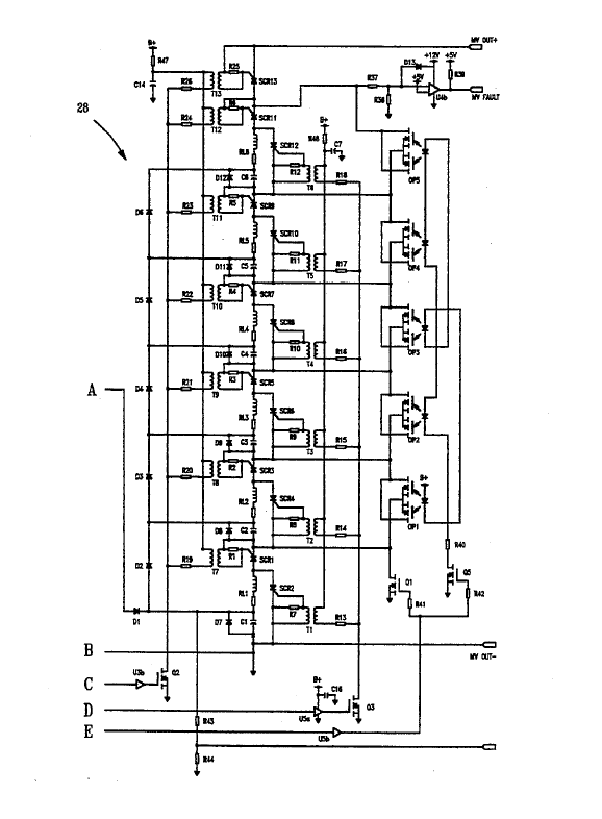
\includegraphics[keepaspectratio=true,scale=1.2,angle=-90]{figuras/circuitodea.eps}
	\caption{Circuito eletrônico DEA. Fonte: \cite{dea}}
	\label{fig:circuitodea}
\end{figure}

\subsubsection{Reanimador Manual}
Para atendimento em urgência, o Reanimador Manual (RM), possibilita eficiente ventilação com ar, sendo este balão auto inflável de vinil.

Um dos recursos a ser utilizado no VANT é o RM, sendo que este produto engloba três categorias, o reanimador recém-nato, infantil e adulto. No projeto serão utilizadas as dimensões do RM infantil e adulto como referência, mas no VANT será utilizado um adaptador com velcro, viabilizando a adequação de cada reanimador, independentes de suas dimensões dentro da margem de tolerância estabelecida.

O RM é usado de acordo com o peso da vítima, se esta tiver menos de 10 kg, o RM a ser designado será o recém-nato, já o RM Infantil é voltado para aqueles entre 10 e 30 Kg. O RM adulto será aplicado a vítimas com 30 Kg ou mais.

Valores utilizados como peso, capacidade do balão entre outros, foram provenientes de informações referentes ao RM da marca Oxigel.

\begin{itemize}
	\item Características
\end{itemize}

\begin{table}[h]
\begin{tabular}{|l|l|l|l|}
\hline
\multicolumn{1}{|c|}{Reanimador} & Capacidade do Balão & Peso & Conexão \\ \hline
Adulto                           & 1200ml              & 410g & 22x15mm \\ \hline
Infantil                         & 500ml               & 210g & 22x15mm \\ \hline
\end{tabular}
\end{table}


\begin{itemize}
	\item Dimensionamento
\end{itemize}

\begin{table}[h]
\begin{tabular}{|l|l|l|l|}
\hline
\multicolumn{1}{|c|}{Reanimador} & Altura & Comprimento & Largura \\ \hline
Adulto                           & 14cm   & 38cm        & 18cm    \\ \hline
Infantil                         & 10cm   & 33cm        & 18cm    \\ \hline
\end{tabular}
\end{table}

\begin{figure}[h!]
	\centering
	  \includegraphics[keepaspectratio=true,scale=0.6]{figuras/animadoradulto.eps}
	\caption{Reanimador Manual Adulto.}
	\label{fig:animadoradulto}
\end{figure}

\begin{figure}[h!]
	\centering
	  \includegraphics[keepaspectratio=true,scale=0.6]{figuras/animadorinfatil.eps}
	\caption{ Reanimador Manual Infantil.}
	\label{fig:animadorinfatil}
\end{figure}

